Los primeros autómatas se desarrollaron en el Antiguo Egipcio. Como es natural estos no tienen nada que ver con lo que hoy se conoce como autómata, pero tenía bastante mérito para la época a la que pertenecen. Eso sí, se consideraban como tales ya que eran capaces de realizar determinadas tareas de forma autónoma. A continuación se van a mencionar los robots más relevantes de la época:\\

 \textbf{Arquitas de Tarento} en el año 400 a.C. diseñó \textit{"la paloma"}[\ref{paloma}], ave mecánica que funcionaba con vapor. El mecanismo era muy rudimentario, debido a la época, y funcionaba de la siguiente manera; Se trataba de un objeto de madera con forma de paloma que se situaba colgada de una cuerda del techo. Esta contenía un pequeño depósito de agua, que se llevaba a ebullición mediante una llama situada en la parte inferior del depósito, y el vapor que se originaba se filtraba por unos pequeños orificios que le permitían al "\textit{robot}" simular el vuelo de la paloma.\\

\begin{figure}[H]
\begin{center}
  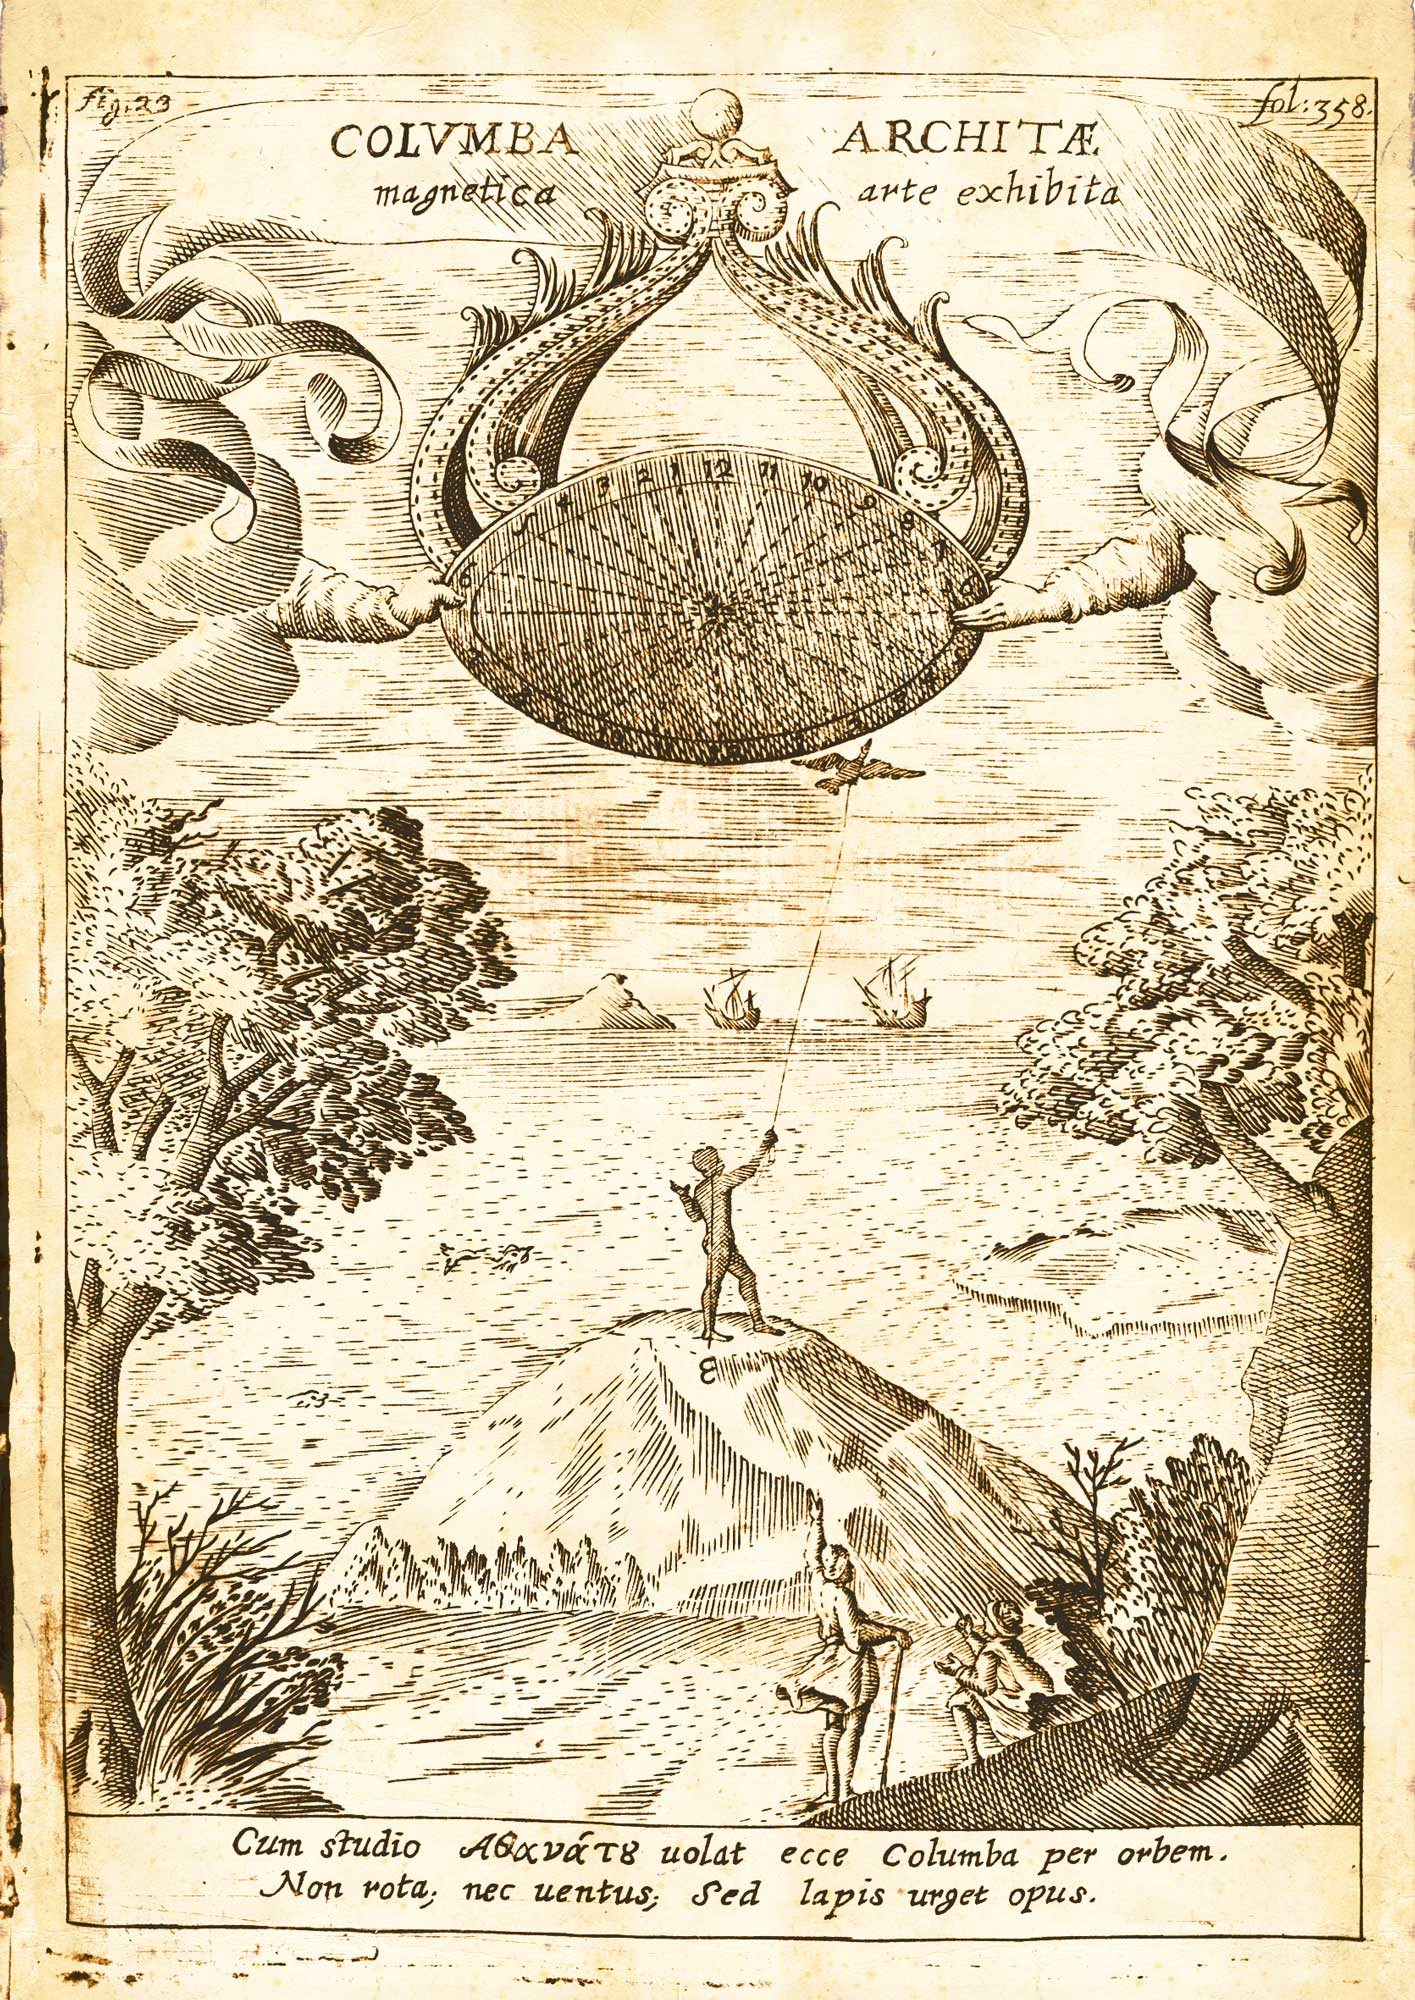
\includegraphics[width=0.5\textwidth]{./EtapaPrimeriza/imagenes/paloma.jpg}
  \caption{Paloma de Arquitas de Tarento (\href{https://www.nationalgeographic.com.es/historia/grandes-reportajes/inventos-griegos_9395/3}{NationalGeographic})}
  \label{paloma}
\end{center}
\end{figure}


\textbf{Apolonio de Pérgamo}, entre 262-190 a.C. , diseñó unos autómatas musicales que funcionaban impulsados por la fuerza del agua.\\


\textbf{Ctesibio de Alejandría}, en el año 300 a.C., también inventó autómatas musicales pero en este caso funcionaban por la propulsión de aire a través de diversos tubos. Pero su contribución más relevante fue el desarrollo del \textit{reloj de agua o clepsidra}, este fue el más preciso de los relojes creados hasta la aparición del reloj de péndulo. Tenía la capacidad de medir el tiempo en función de lo que tarda en caer el agua de un recipiente a otro. Hasta ese momento, el tiempo se medía el tiempo a través de la observación del movimiento del sol, lo que no permitía medir el tiempo en cualquier momento del día. A continuación se muestra una imagen de dicho reloj:\\


\begin{figure}[H]
\begin{center}
  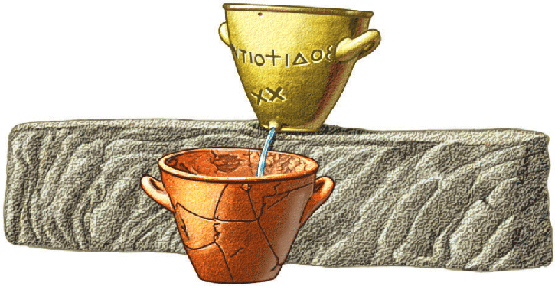
\includegraphics[width=0.5\textwidth]{./EtapaPrimeriza/imagenes/reloj.png}
  \caption{Reloj de Agua de Ctesibio de Alejandría (\href{http://quhist.com/origen-a-lo-largo-historia-termino-clepsidra/}{QuHist})}
  \label{reloj}
\end{center}
\end{figure}



\textbf{Filón de Bizancio} inventa en el año 200 a. C., hizo numerosas contribuciones a la ciencia que se describirán a continuación. Uno de los inventos más revolucionarios fue el molino de agua que se utilizaba tanto para moler grano como para diversos trabajos agrícolas. Además, ideó la bomba de agua que permitía transportar el agua desde un nacimiento hasta una zona geográficamente más alta mediante la fuerza de la propia agua. Relacionado también con el agua, ideó un lavabo en el que, como se puede ver en la siguiente imagen, contenía en su parte superior un recipiente lleno de agua. Esta agua caía sobre un cucharón situado bajo el mismo y cuando se llenaba se inclinaba y el agua caía sobre el grifo y pudiendo obtenerla de forma dosificada. Al mismo tiempo que el agua caía por el grifo, también se dejaba caer una pequeña piedra pómez para limpiarte.\\


\begin{figure}[H]
\begin{center}
  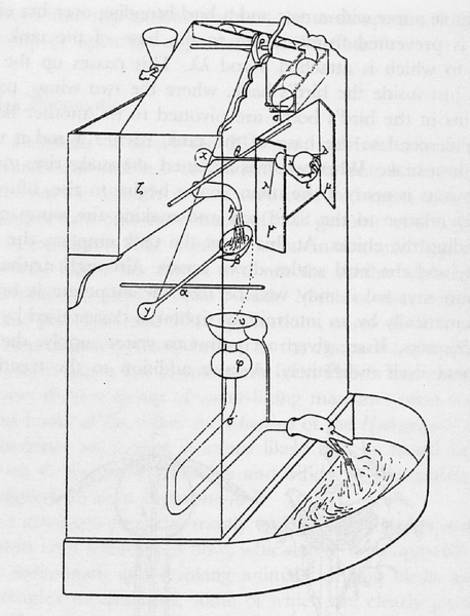
\includegraphics[width=0.3\textwidth]{./EtapaPrimeriza/imagenes/lavabo.jpg}
  \caption{Lavabo de Filón de Bizancio (\href{http://historiautomatas.blogspot.com/2010/06/grecia-ii-filon-de-bizancio.html} {HistoriaAutómatas})}
  \label{lavabo}
\end{center}
\end{figure}

Pero estas no fueron las únicas contribuciones de Filón de Bizancio. Tenía cierto interés por el tema armamentístico y es por ello que diseñó las primeras flechas, una ballesta que está compuesta por dos cadenas unidas con una polea tal que se lanzaban flechas mientras le quedaran en la recámara. Y por último, y uno de sus inventos más curiosos fue lo que se llamó una \textit{camarera automática}. Esto era una estatua que tenía colocada en una de sus manos una jarra y cuando se le colocaba en la otra mano un vaso, esta cedía por el peso y el tubo que conectaba la jarra con el depósito del vino se accionaba para llenar el vaso.



\textbf{Herón de Alejandría} destaca por las numerosas contribuciones que hizo a la ciencia en la antigüedad. Es por ello que se va a hacer desarrollar sus contribuciones más relevantes y algunas de ellas han facilitado avances industriales a lo largo de la historia.

En sus contribuciones a lo que podría ser la robótica de la época se destaca su trabajo conocido como \textit{Mecánica}, en el que se plasman los primeros datos descriptivos acerca de la construcción de un autómata. Está compuesto por tres libros en los que se trata de las proporciones de las figuras en el primero de ellos, en el segundo de los sistemas mecánicos simples que son descritos en el siguiente apartado y finalmente en su último libro hablaba sobre las aplicaciones de la mecánica.

Cuando hablamos de inventos concretos se destaca que creó la primera máquina de vapor de la historia a la que llamaron \textit{eolípila}. Esta estaba compuesta por una caldera de agua hirviendo y sobre esta se situaba una esfera hueca llena de agua conectadas ambas cosas por dos tubos como se ve en la siguiente imagen [\ref{mv}]. Cuando el agua hervía se conseguía que la esfera girase a gran velocidad. En la época se dice que solo servía como un divertimento para los niños pero la realidad es que en el futuro serviría como inspiración a las máquinas de vapor utilizadas en las industrias.

\begin{figure}[H]
\begin{center}
  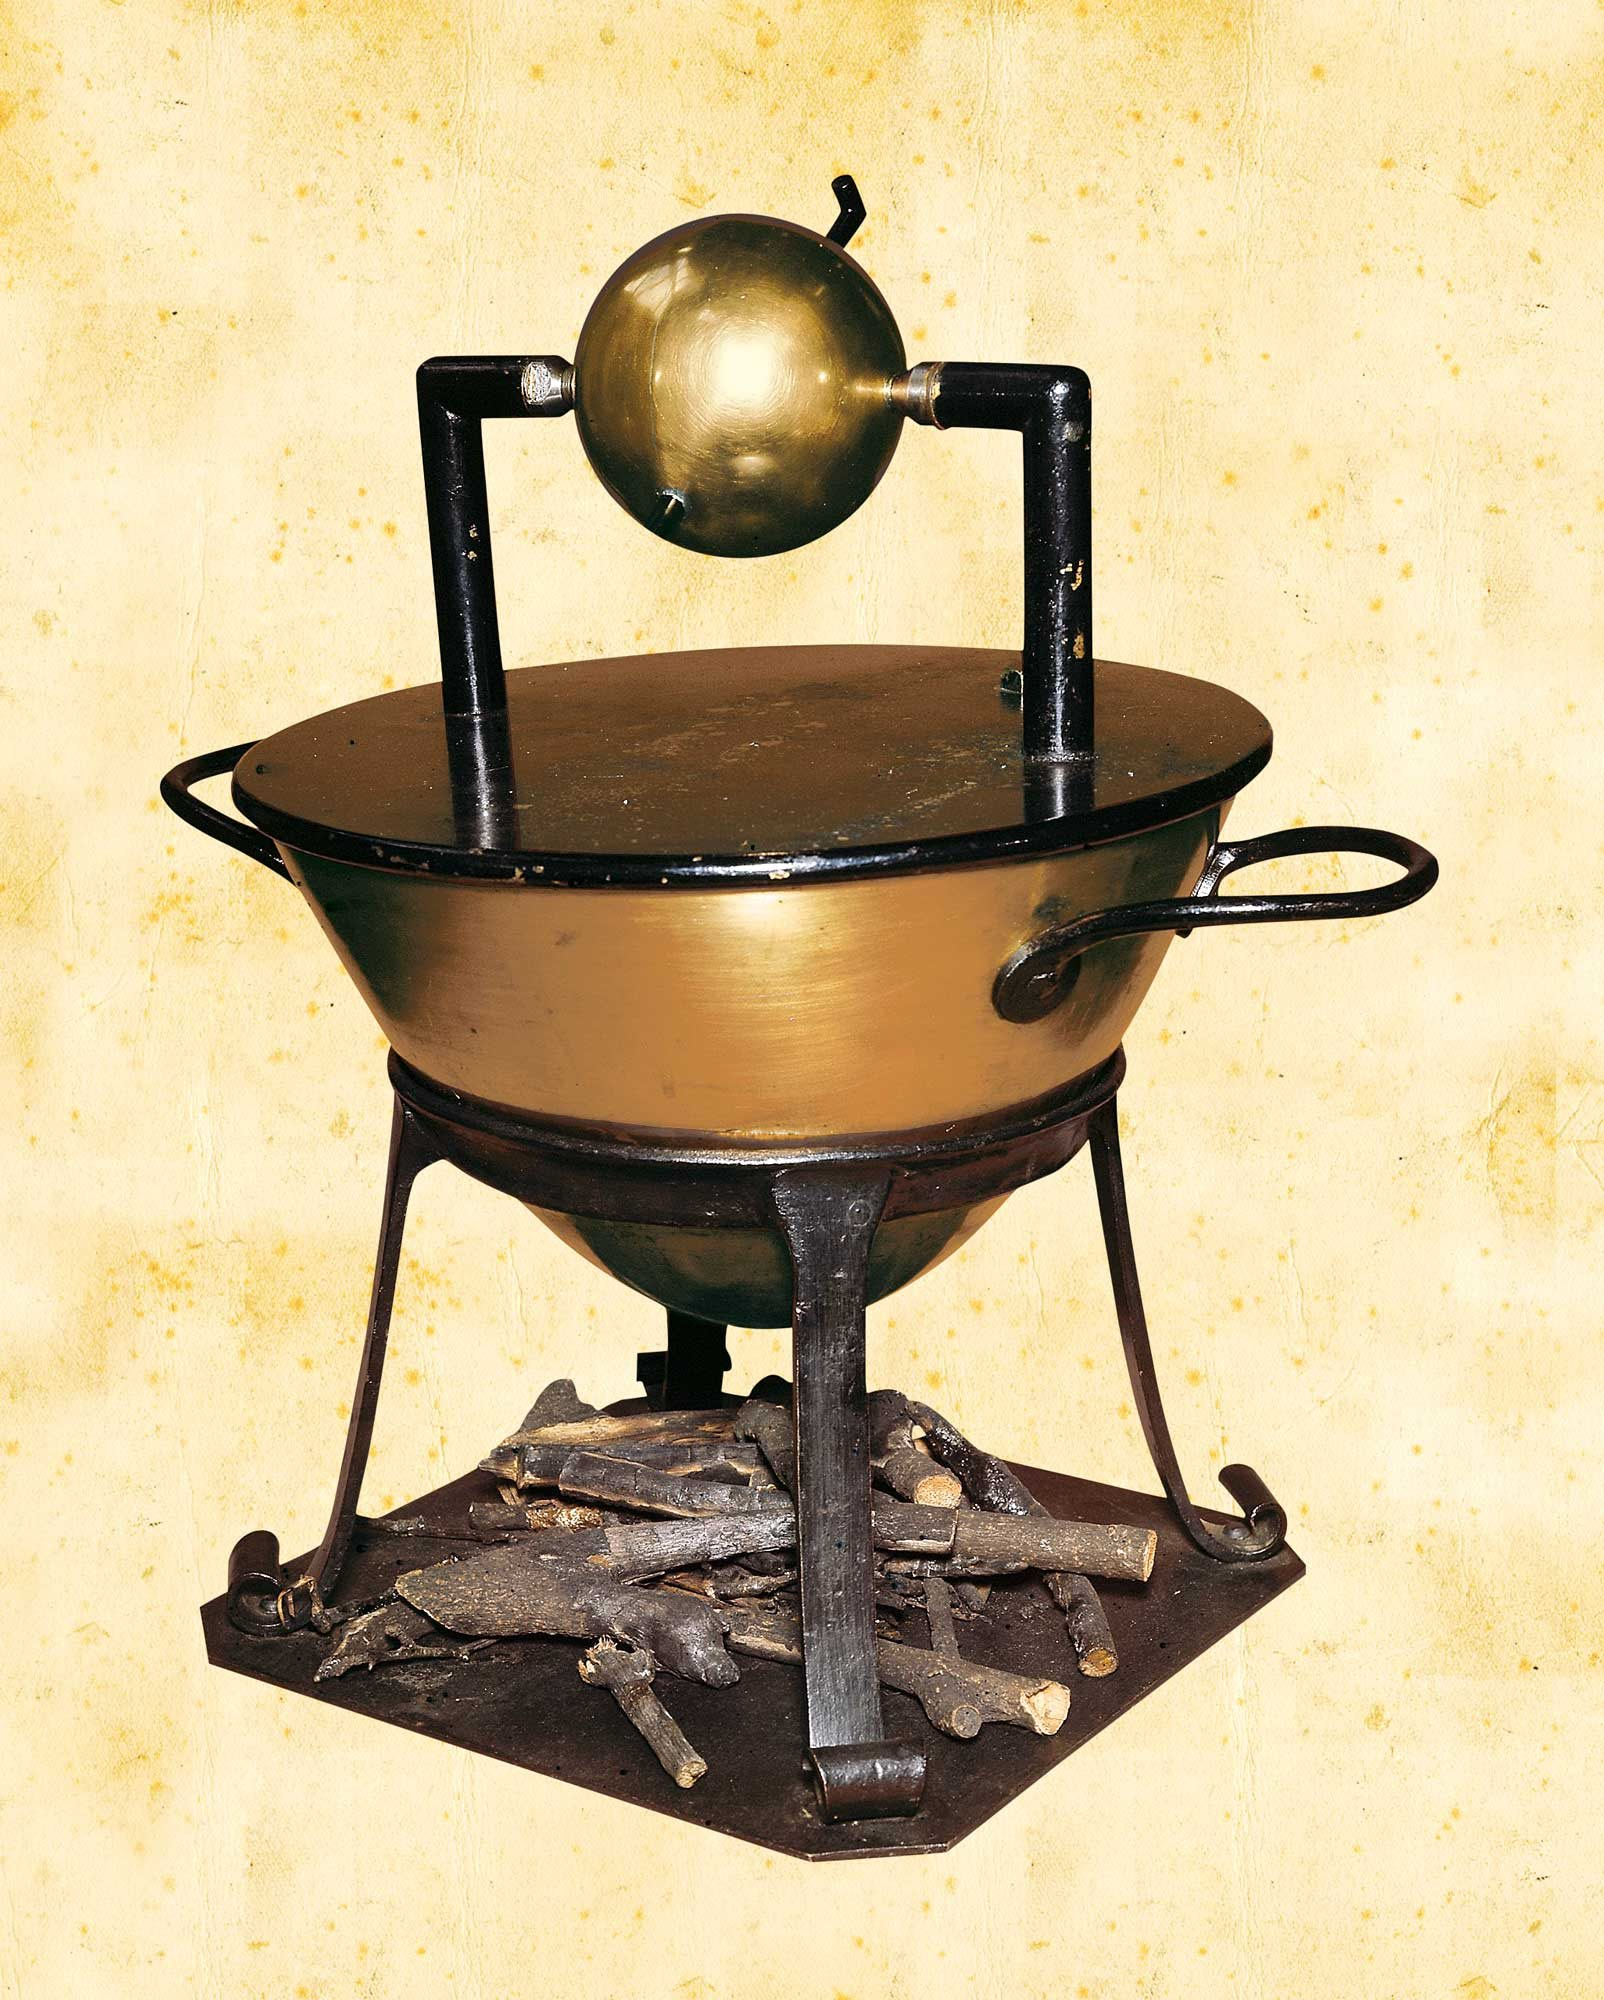
\includegraphics[width=0.3\textwidth]{./EtapaPrimeriza/imagenes/mv.jpg}
  \caption{Eolípila de Herón (\href{https://www.nationalgeographic.com.es/historia/grandes-reportajes/inventos-griegos\_9395}{NationalGeographic})}
  \label{mv}
\end{center}
\end{figure}

Además diseñó lo que fueron los primeros autómatas y las primeras puertas automáticas. Con la energía que proporcionaba la \textit{eolípila} y con sistemas mecánicos simples como cuerdas, poleas, cadenas y demás era capaz de poner en movimiento autómatas y puertas automáticas. La realidad es que no existe constancia de que lo llevara acabo pero la idea si que la tuvo y dejó constancia de ello en sus libros.\\


En el 770 d. C., \textbf{Yang Wu-Lien } diseñó un prototipo con forma de mono que alargaba la mano para que le dieran limosna. Cuando la mano alcanzaba un cierto peso, este guardaba el dinero en una bolsa.\\



En el 890, \textbf{Han Chih Ho} creó un gato de madera que se encargaba de cazar ratas y ratones que hubiese a su alrededor.\\

El príncipe hindú \textbf{Bhoja}, en el año 1050, escribió \textit{Samarangana-Sutradhara} donde se describe cómo es el proceso de construcción de máquinas que eran capaces de actuar autónomamente y que se las llamaba \textit{yantras}.\\


Pero la realidad es que, en la antigüedad, las máquinas más perfectas que se consiguieron fueron los relojes ya que se acercaban al concepto de automatismo y por consiguiente al de robótica. Algunos de ellos cuentan con figuras humanas que sus movimientos van en función del transcurso de las horas. Ejemplos de ello son los relojes de la catedral de Múnich y el reloj de Ánker que se puede visitar en la ciudad de Viena, Austria.

Más concretamente, en España se conserva un reloj construido en el siglo XVI, llamado Papamoscas,  y que está compuesto por un hombre que se mueve con los cambios horarios. Hoy en día sigue funcionado y se puede visitar en la catedral de Burgos.


Aunque se ha de señalar que el robot más antiguo, que estuvo en funcionamiento entre 1352 y 1789, y que se conserva en la actualidad es el Gallo de Estrasburgo. Este formaba era parte del reloj de la catedral de Estrasburgo y hacía mover sus alas y su pico al dar las horas.

\begin{figure}[H]
\begin{center}
  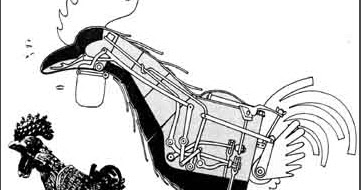
\includegraphics[width=0.3\textwidth]{./EtapaPrimeriza/imagenes/gallo.jpg}
  \caption{Gallo de Estrasburgo  (\href{http://lasmilrespuestas.blogspot.com/2012/06/como-funcionaban-los-automatas.html} {Autómatas})}
  \label{gallo}
\end{center}
\end{figure}


Finalmente, para terminar con los orígenes de la robótica no podemos dejar de nombrar "\textit{el hombre de hierro}" de Alberto Magno del siglo XIII. Este era un autómata con forma de humano construido con hierro, cristal y cuero y que era capaz caminar, abrir puertas, entretener invitados y hasta incluso hacer tareas del hogar. Este es considerado como el inicio de lo que hoy en día es la inteligencia artificial.
